\newpage


\textbf{a)} Analizando paso por paso el primer inciso \ref{a}, se puede resolver en dos partes \textbf{(I - II')} y \textbf{(III' $\cap$ II)'} para así unir ambos subconjuntos \\

Resolviendo \textbf{(I - II')}

\begin{align*}
(I - I')  &= \{a, e, i, o, u\} - \{ a, b, c, d, e, f, g, i, k, l, m, n, o, t, u, v, w, x, y, z \}  \\
  &= \{\} \\
\end{align*}

Resolviendo \textbf{(III' $\cap$ II)'}

\begin{align*}
(III' \cap II)'  &= \{ k, l, m, n, p, q, r, s, t, v, w, x, y, z \} \cap (\{ h, j, p, q, r, s  \})'  \\
  &= (\{p, q, r, s \} )'\\
\end{align*}

Juntando ambos lados para armar (I - II') $\cup$ (III' $\cap$ II)':

\begin{align*}
(I - II') \cup (III' \cap II)' &= ( \{ \} \cup \{p, q, r, s \} )' \\
  &= \{p, q, r, s \}' \\
  &= \{ a, b, c, d, e, f, g, h, i, j, k, l, m, n, o, t, u, v, w, x, y, z \} 
\end{align*}

Por lo tanto el resultado es

\begin{equation*}
    \boxed{(I - II') \cup (III' \cap II)' = \{ a, b, c, d, e, f, g, h, i, j, k, l, m, n, o, t, u, v, w, x, y, z \} }
\end{equation*}

Para obtener el diagrama de Venn, se puede hacer por partes, el lado derecho y lado izquierdo, quedando: \\

\textbf{(I - II')}: 

\begin{figure}[htbp]
\centering
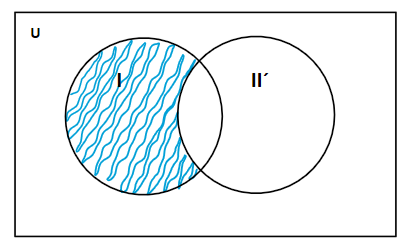
\includegraphics[width=8cm]{a/aa.png}
\caption[]{Diagrama de Venn de (I - II')}
\end{figure} 

\newpage

\textbf{(III' $\cap$ II)'}:

\begin{figure}[htbp]
\centering
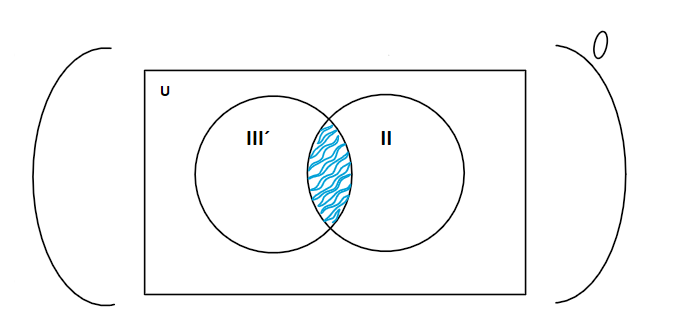
\includegraphics[width=8cm]{a/bb.png}
\caption[]{Diagrama de Venn de (III' $\cap$ II)'}
\end{figure} 

Sacando el complemento, queda el diagrama

\begin{figure}[htbp]
\centering
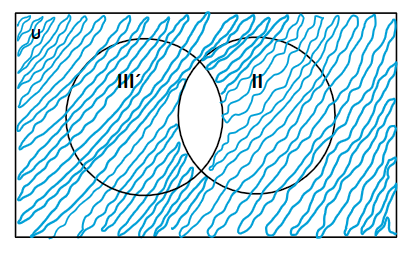
\includegraphics[width=8cm]{a/bbb.png}
\caption[]{Diagrama de Venn de (III' $\cap$ II)'}
\end{figure} 

Haciendo la unión de ambos lados para armar (I - II') $\cup$ (III' $\cap$ II)', quedando así el diagrama de Venn:

\begin{figure}[htbp]
\centering
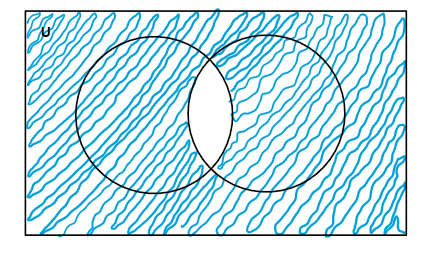
\includegraphics[width=8cm]{a/aabb.png}
\caption[]{Diagrama de Venn de (I - II') $\cup$ (III' $\cap$ II)'}
\end{figure} 